\begin{figure}[htbp]
\centering
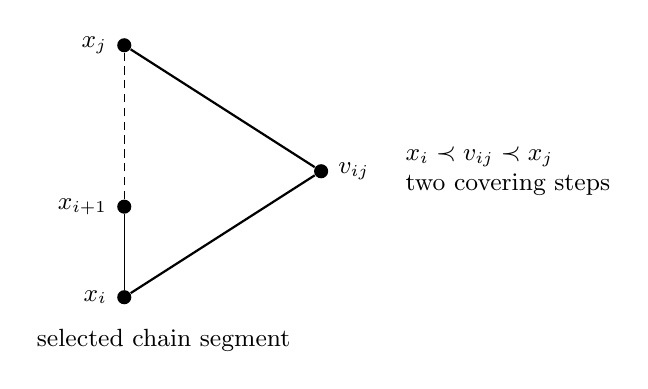
\begin{tikzpicture}[x=1cm,y=1cm,
  vertex/.style={circle,fill=black,inner sep=1.8pt},
  every node/.style={font=\small}]
\node[vertex,label=left:{$x_i$}] (lo) at (0,0) {};
\node[vertex,label=left:{$x_{i+1}$}] (mid) at (0,1.15) {};
\node[vertex,label=left:{$x_j$}] (hi) at (0,3.2) {};
\node[vertex,label=right:{$v_{ij}$}] (shortcut) at (2.5,1.6) {};
\draw (lo)--(mid);
\draw[densely dashed] (mid)--(hi);
\draw[thick] (lo)--(shortcut)--(hi);
\node[align=left,anchor=west] at (3.45,1.6)
  {$x_i\prec v_{ij}\prec x_j$\\two covering steps};
\node[align=center] at (0.5,-.55) {selected chain segment};
\end{tikzpicture}
\caption{One shortcut in a tested chain. The two thick edges are covers
in the entire subgroup interval; the selected chain on the left can
have arbitrarily many intermediate vertices and is not required to be
saturated. Fences, coatom witnesses, and the $M_{16}$ tests are omitted.
The proof compares the restrictions imposed by every short route with
those imposed by traversing a long chain.}
\label{fig:tested-chain}
\end{figure}
